\def\checkmark{\tikz\fill[scale=0.4](0,.35) -- (.25,0) -- (1,.7) -- (.25,.15) -- cycle;}

\chapter{\ifproject%
      \ifenglish Experimentation and Results\else การทดลองและผลลัพธ์\fi
  \else%
      \ifenglish System Evaluation\else การประเมินระบบ\fi
  \fi}

ในการทดลองนี้เราจะใช้ระบบของเราในการทำการทดสอบโดยจะทำการทดสอบโดยใช้เงินตั้งต้น 3,000 USD และทดสอบบนตลาด Crypto Currency (BTC, ETH, BNB) และตลาดหุ้น NASDAQ (AAPL, IBM, JPM, MSFT, NKE, TSLA) ซึ่งเงินตั้งต้นจะถูกแบ่งให้เท่าๆ กันจาก 3,000 USD สำหรับแต่ละเหรียญหรือหุ้นในทั้ง 2 ตลาด โดยวิธีการเข้าซื้อจะมีดังนี้

\begin{table}[ht]
    \centering
    \resizebox{\columnwidth}{!}{%
        \begin{tabular}{lccccc}
            \textbf{ส่วนเสริม}                                                                                                         &
            \multicolumn{1}{l}{\textbf{Classical}}                                                                                   &
            \multicolumn{1}{l}{\textbf{Fuzzy}}                                                                                       &
            \multicolumn{1}{l}{\textbf{Fuzzy C}}                                                                                     &
            \multicolumn{1}{l}{\textbf{Fuzzy PSO}}                                                                                   &
            \multicolumn{1}{l}{\textbf{Fuzzy PSO}}                                                                                                                                           \\
            ใช้ Fuzzy Logic ในการทำอินดิเคเตอร์ขึ้นมา                                                                                       &   & \checkmark &            & \checkmark & \checkmark \\
            \begin{tabular}[c]{@{}l@{}}การจัดการเงินทุนโดยใช้ค่าของอินดิเคเตอร์จาก  Fuzzy Logic\\ (Liquidation F)\end{tabular}               &   &            & \checkmark &            & \checkmark \\
            \begin{tabular}[c]{@{}l@{}}การใช้ Particle Swarm Optimization (PSO) ในการปรับค่าของตัว\\ แปรทางภาษาของอินดิเคเตอร์\end{tabular} &   &            &            & \checkmark & \checkmark
        \end{tabular}%
    }
    \caption{ตัวชี้วัดที่นำมาใช้ในการเข้าซื้อ}
    \label{tab:indicators}
\end{table}
โดยสำหรับวิธี Classical นั้นเราจะใช้ค่าของอินดิเคเตอร์แต่ละตัวตรงๆ มาใช้ตัดสินใจเข้าซื้อ ส่วนด้านล่างนี้เป็นเงื่อนไขสำหรับการทดสอบ
%และสำหรับการใช้ PSO เราจะใช้ข้อมูล ตั้งแต่จุดเริ่มต้นต้นของแต่ละตลาดถึงเดือนมีนาคม 2023 ในการฝึกสอน แล้วในเดือนเมษายน 2023 ถึงเดือนกันยายน 2023 จะเป็นช่วงของการทดสอบและเลือกการปรับค่าที่ดีที่สุด

\begin{itemize}
    \item {มีการเข้าซื้อขั้นต่ำอยู่ที่ 30 USD}
    \item {สำหรับการเข้าซื้อแบบที่ไม่ได้การจัดการเงินทุนจะเข้าซื้อที่ 5\% ของเงินที่มีอยู่ขณะนั้น}
    \item {สำหรับตลาด Crypto Curreny เมื่อกำไรของการเข้าซื้อนั้น ≥ 20\% (take profit) หรือเมื่อขาดทุน ≥ 10\% (stop loss) เราจะขายออก}
    \item {สำหรับตลาดหุ้น NASDAQ เมื่อกำไรของการเข้าซื้อนั้น ≥ 10\% (take profit) หรือเมื่อขาดทุน ≥ 5\% (stop loss) เราจะขายออก}
\end{itemize}
นอกจากนี้เราจะมีวิธี Buy \& Hold ซึ่งเป็นวิธีการนี้ก็คือการซื้อสินทรัพย์ไว้ด้วยจำนวนเงินทั้งหมด ตั้งแต่วันแรกที่ทดสอบไว้แล้วถือไว้โดยไม่ขายออกเป็นตัวไว้เปรียบเทียบ การทดสอบจะเริ่มตั้งแต่วันที่ 1 ตุลาคม 2023 ถึง 8 มีนาคม 2024 เป็นเวลาประมาณ 5 เดือน

\section{พารามิเตอร์ในการใช้ PSO}
ในการใช้ PSO เราจะกำหนดให้มีพารามิเตอร์ตังนี้
\begin{itemize}
    \item {จำนวนกลุ่ม (Swarm Size) ที่ใช้ในการฝึกสอน จะมี 3 รูปแบบ คือ 5, 10, 15}
    \item {จำนวนสมาชิกในแต่ละกลุ่ม (Number of Particles) จะเป็น 10}
    \item {เงื่อนไขในการจบการทำงาน คือเมื่อถึงรอบที่ 10}
\end{itemize}
โดยเราจะฝึกสอนโดยใช้ข้อมูลตั้งแต่จุดเริ่มต้นของข้อมูลตลาดแต่ละตลาด ถึงจุดเริ่มต้นของช่วง validation ซึ่งจะเป็น 6 เดือนก่อนหน้าวันที่ 1 ตุลาคม 2023 และเราก็จะใช้กรอบเวลาของข้อมูลเป็นสี่ชั่วโมง (4h) จากนั้นเราก็จะเลือกตัวที่ให้ผลลัพธ์ที่ดีที่สุด แล้วไปใช้ในการทดสอบต่อไป

\iffalse
    Timeframe 1h or 1d, or we should just use 1d to make it faster, if we know the current market trend, bullish or bearish
    and long on buliish only, short on bearish only -> we will gain much more profit
\fi

\section{AROON-MACD}
สำหรับตัวชี้วัดตัวนี้จะมีตัวแปรทางภาษาตามรูปที่ \ref{fig:aroon-macd-lin} ในภาคผนวก และมี Fuzzy Rules ดังรูปที่ \ref{fig:aroon-macd-rules} ด้านล่างนี้
\begin{figure}[!ht]
    \centering
    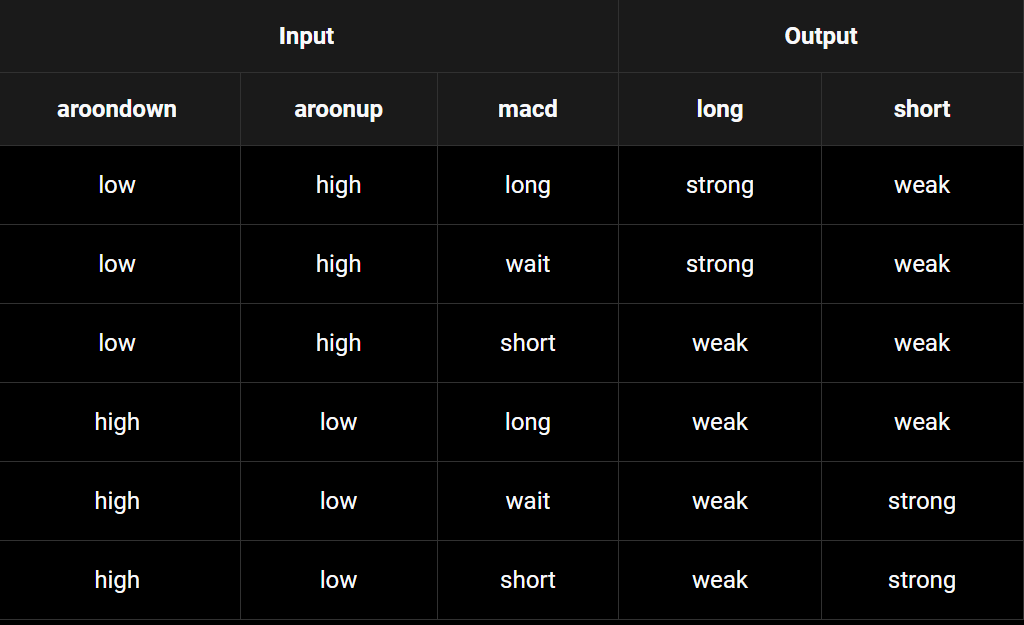
\includegraphics[width=\textwidth]{images/aroon-macd-rules.png}
    \caption{Fuzzy Rules ของตัวชี้วัด AROON-MACD จากในระบบของเรา}
    \label{fig:aroon-macd-rules}
\end{figure}

โดยสำหรับตัวชี้วัดนี้จะเป็นตัวชี้วัดแบบ Trend Following ซึ่งคือการที่เราพยายามซื้อขายสินทรัพย์ตามแนวโน้มของตลาด ถ้าตลาดกำลังอยู่ในขาขึ้นก็จะมีการทำการเข้าซื้อแบบ long และถ้าตลาดกำลังอยู่ในขาลงก็จะมีการทำการเข้าซื้อแบบ short โดย MACD จะเป็นตัวที่บอกเราว่าควรเข้าซื้อ ณ เวลาไหน และ AROON จะเป็นตัวบอกเราว่าตลาดกำลังอยู่ในขาขึ้นหรือขาลง โดยเราจะเข้าซื้อเมื่อค่าของอินดิเคเตอร์มีค่าเกิน 30

\begin{table}[!h]
    \centering
    \begin{tabular}{crrrrr}
        \hline
        \textbf{Symbol} & \textbf{Classical} & \textbf{Fuzzy} & \textbf{Fuzzy C} & \textbf{Fuzzy PSO} & \textbf{Fuzzy PSO C} \\ \hline
        BTC             & 680.48             & 654.28         & 1035.67          & 1383.01            & \textbf{1450.66}     \\ \hline
        ETH             & 440.45             & 509.39         & 509.16           & 294.08             & \textbf{1264.20}     \\ \hline
        BNB             & 448.98             & 496.05         & 736.79           & 554.83             & \textbf{926.30}      \\ \hline
        TOTAL           & 1569.91            & 1659.72        & 2281.62          & 2231.92            & \textbf{3641.15}     \\ \hline
    \end{tabular}
    \caption{ผลกำไรขาดทุนของการทดสอบตัวชี้วัด AROON-MACD ในตลาด Crypto Currency (หน่วยเป็น USD)}
    \label{tab:aroon-macd-crypto}
\end{table}

\begin{figure}[!h]
    \centering
    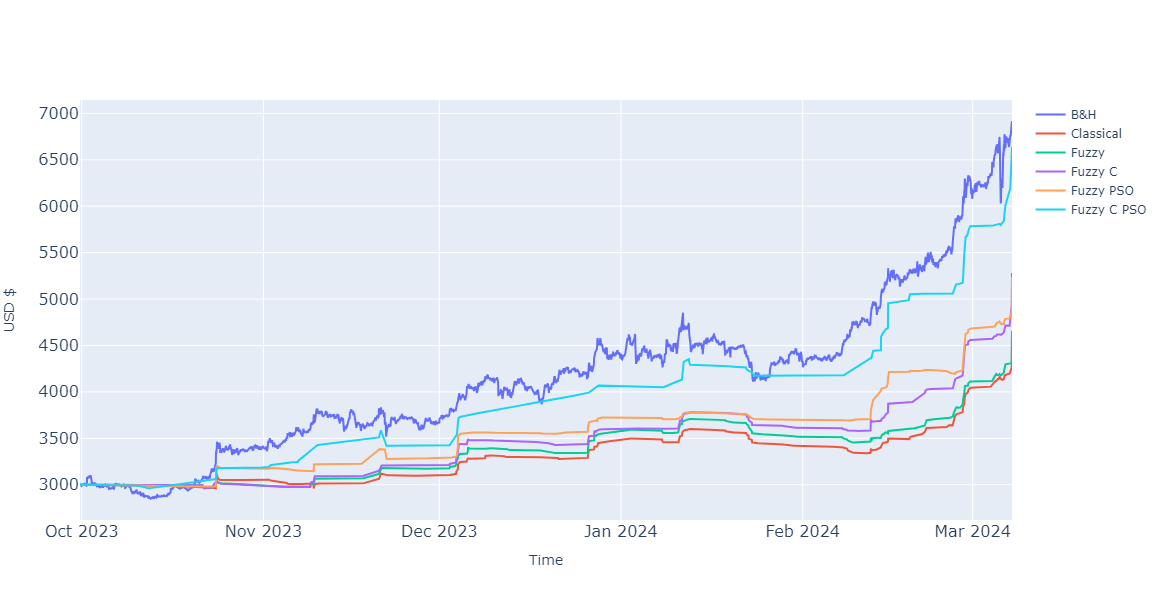
\includegraphics[width=\textwidth]{images/aroon-macd/crypto-result.png}
    \caption{ความเปลี่ยนของเงินลงทุนของตัวชี้วัด AROON-MACD ในตลาด Crypto Currency}
    \label{fig:aroon-macd-crypto}
\end{figure}

\begin{table}[!h]
    \centering
    \begin{tabular}{crrrrr}
        \hline
        \textbf{Symbol} & \textbf{Classical} & \textbf{Fuzzy} & \textbf{Fuzzy C} & \textbf{Fuzzy PSO} & \textbf{Fuzzy PSO C} \\ \hline
        AAPL            & \textbf{4.41}      & 0.37           & -0.01            & -18.55             & -23.70               \\ \hline
        IBM             & \textbf{81.12}     & 62.58          & 28.71            & 74.48              & 75.30                \\ \hline
        JPM             & 13.59              & \textbf{20.73} & 20.72            & 7.41               & -10.78               \\ \hline
        MSFT            & \textbf{90.80}     & 64.01          & 64.80            & 59.54              & 6.60                 \\ \hline
        NKE             & \textbf{45.31}     & 23.76          & 23.68            & 23.71              & -27.81               \\ \hline
        TSLA            & \textbf{171.23}    & 59.16          & 56.97            & 6.73               & -3.14                \\ \hline
        TOTAL           & \textbf{406.46}    & 230.62         & 194.87           & 153.30             & 16.47                \\ \hline
    \end{tabular}
    \caption{ผลกำไรขาดทุนของการทดสอบตัวชี้วัด AROON-MACD ในตลาดหุ้น NASDAQ (หน่วยเป็น USD)}
    \label{tab:aroon-macd-stocks}
\end{table}

\begin{figure}[!h]
    \centering
    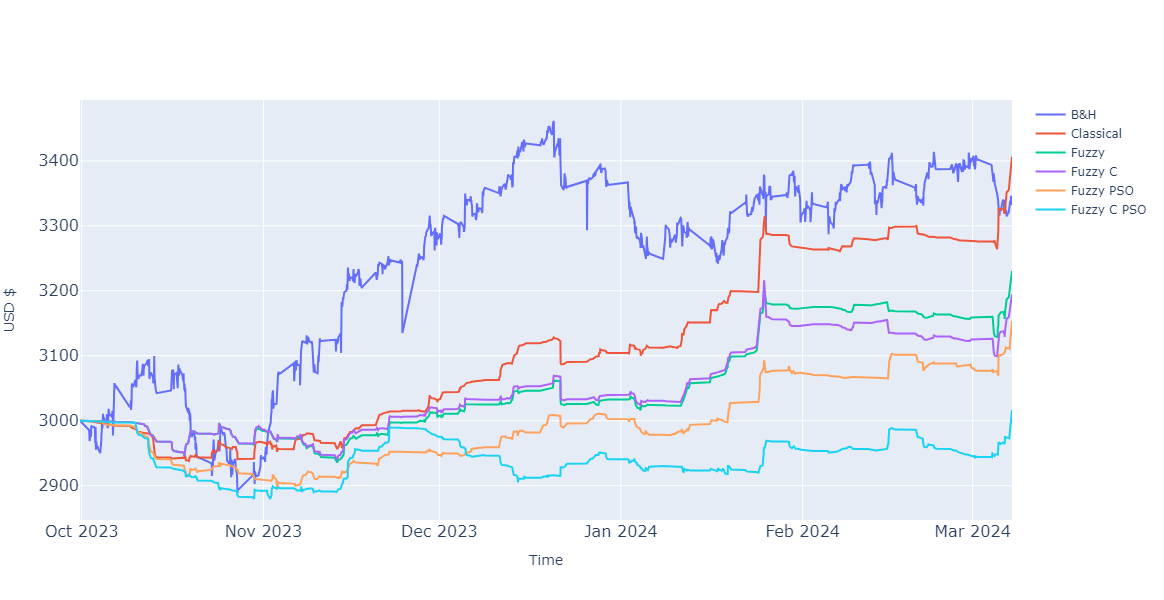
\includegraphics[width=\textwidth]{images/aroon-macd/stock-result.png}
    \caption{ความเปลี่ยนของเงินลงทุนของตัวชี้วัด AROON-MACD ในตลาดหุ้น NASDAQ}
    \label{fig:aroon-macd-stock}
\end{figure}

จากตารางที่ \ref{tab:aroon-macd-crypto} และรูปที่ \ref{fig:aroon-macd-crypto} เราจะเห็นว่าการใช้ตัวชี้วัดที่ใช้ Fuzzy Logic นั้นให้ผลลัพธ์ที่ดีกว่าแบบ Classical ในตลาด Crypto Currency แต่ในตารางที่ \ref{tab:aroon-macd-stocks} และรูปที่ \ref{fig:aroon-macd-stock}

\section{RSI-BB}
สำหรับตัวชี้วัดตัวนี้จะมีตัวแปรทางภาษาตามรูปที่ \ref{fig:rsi-bb-lin} ในภาคผนวก และมี Fuzzy Rules ดังรูปที่ \ref{fig:rsi-bb-rules} ด้านล่างนี้
\begin{figure}[!ht]
    \centering
    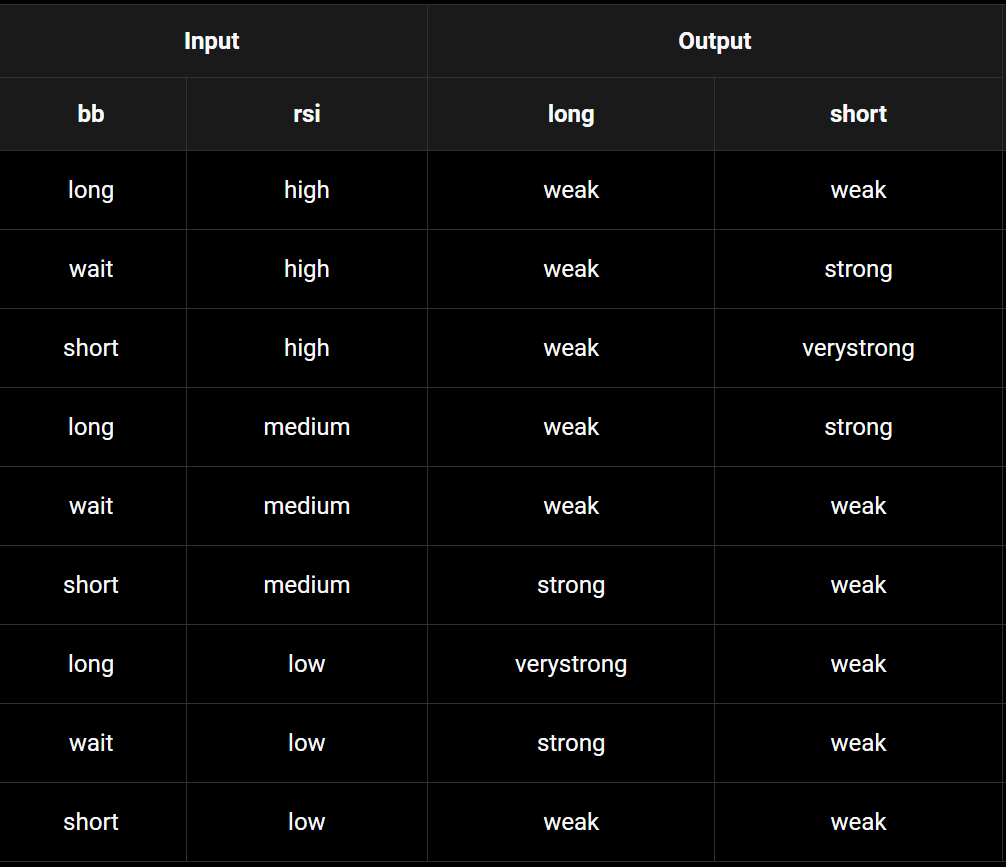
\includegraphics[width=0.8\textwidth]{images/rsi-bb-rules.png}
    \caption{Fuzzy Rules ของตัวชี้วัด RSI-BB จากในระบบของเรา}
    \label{fig:rsi-bb-rules}
\end{figure}

โดยสำหรับตัวชี้วัดนี้จะเป็นตัวชี้วัดแบบ Mean Reversion ซึ่งคือการที่เราคาดว่าราคาของสินทรัพย์จะมีแนวโน้มที่จะกลับมาสู่ราคาเฉลี่ย โดย bollinger band (bb) จะเป็นตัวบอกว่าราคาของสินทรัพย์นั้นสูงหรือต่ำกว่าค่าเฉลี่ยเกินไปหรือไม่ และ rsi จะเป็นตัวที่บอกเราว่าควรเข้าซื้อ ณ ตอนไหน ถ้าราคาของสินทรัพย์นั้นต่ำกว่าค่าเฉลี่ย และ rsi บอกว่าสินทรัพย์นั้นมีการขายอย่างมาก เราก็จะเข้าซื้อแบบ long และถ้าราคาของสินทรัพย์นั้นสูงกว่าค่าเฉลี่ย และ rsi บอกว่าสินทรัพย์นั้นมีการซื้ออย่างมาก เราก็จะเช้าซื้อแบบ short โดย เราจะเข้าซื้อเมื่อค่าของอินดิเคเตอร์รี้มีค่าเกิน 25

\begin{table}[!ht]
    \centering
    \begin{tabular}{crrrrr}
        \hline
        \textbf{Symbol} & \textbf{Classical} & \textbf{Fuzzy} & \textbf{Fuzzy C} & \textbf{Fuzzy PSO} & \textbf{Fuzzy PSO C} \\ \hline
        BTC             & -110.64            & -105.57        & -96.40           & 1381.81            & \textbf{1466.41}     \\ \hline
        ETH             & -84.48             & -24.46         & -49.72           & \textbf{1261.53}   & -49.72               \\ \hline
        BNB             & -109.26            & 28.17          & 20.36            & 28.17              & \textbf{1044.98}     \\ \hline
        TOTAL           & -304.38            & -101.87        & -125.76          & \textbf{2671.50}   & 2461.67              \\ \hline
    \end{tabular}
    \caption{ผลกำไรขาดทุนของการทดสอบตัวชี้วัด RSI-BB ในตลาด Crypto Currency (หน่วยเป็น USD)}
    \label{tab:rsi-bb-crypto}
\end{table}

\begin{figure}[!ht]
    \centering
    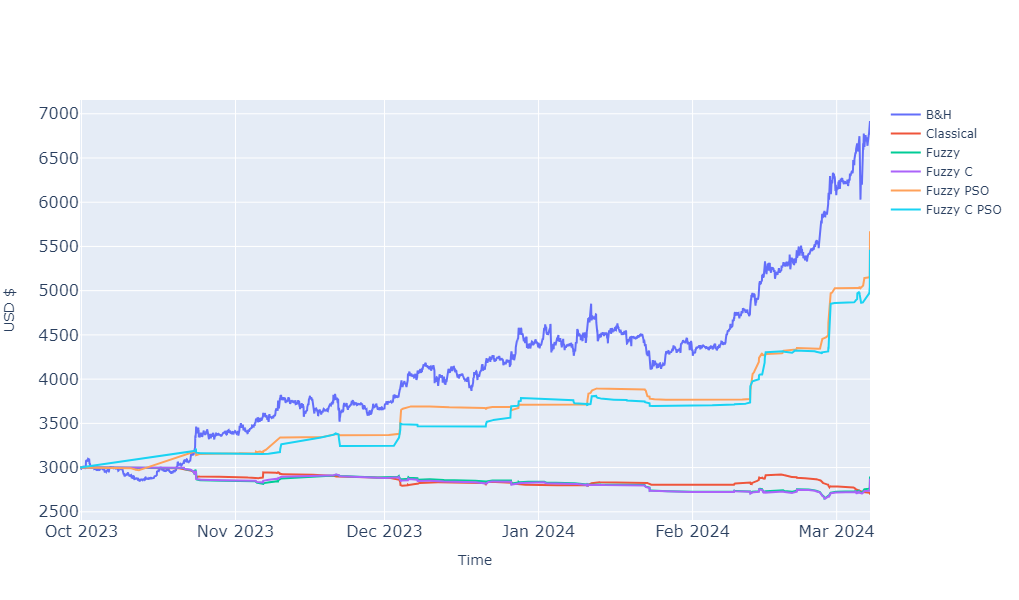
\includegraphics[width=\textwidth]{images/rsi-bb/crypto-result.png}
    \caption{ความเปลี่ยนของเงินลงทุนของตัวชี้วัด RSI-BB ในตลาด Crypto Currency}
\end{figure}

\begin{table}[!ht]
    \centering
    \begin{tabular}{crrrrr}
        \hline
        \textbf{Symbol} & \textbf{Classical} & \textbf{Fuzzy} & \textbf{Fuzzy C} & \textbf{Fuzzy PSO} & \textbf{Fuzzy PSO C} \\ \hline
        AAPL            & \textbf{17.09}     & -20.55         & -20.55           & -21.33             & -3.53                \\ \hline
        IBM             & -50.07             & 69.16          & 53.64            & \textbf{172.27}    & 17.32                \\ \hline
        JPM             & -57.70             & \textbf{24.27} & 20.96            & -112.47            & -109.25              \\ \hline
        MSFT            & -25.98             & 37.86          & 41.21            & \textbf{89.50}     & -15.32               \\ \hline
        NKE             & -7.20              & -45.88         & -45.88           & -45.88             & -22.72               \\ \hline
        TSLA            & -14.12             & \textbf{2.70}  & \textbf{2.70}    & -64.64             &
        \textbf{2.70}                                                                                                        \\ \hline
        TOTAL           & -137.99            & \textbf{67.56} & 52.08            & 17.45              & -130.80              \\ \hline
    \end{tabular}
    \caption{ผลกำไรขาดทุนของการทดสอบตัวชี้วัด RSI-BB ในตลาดหุ้น NASDAQ (หน่วยเป็น USD)}
    \label{tab:rsi-bb-stocks}
\end{table}

\begin{figure}[!ht]
    \centering
    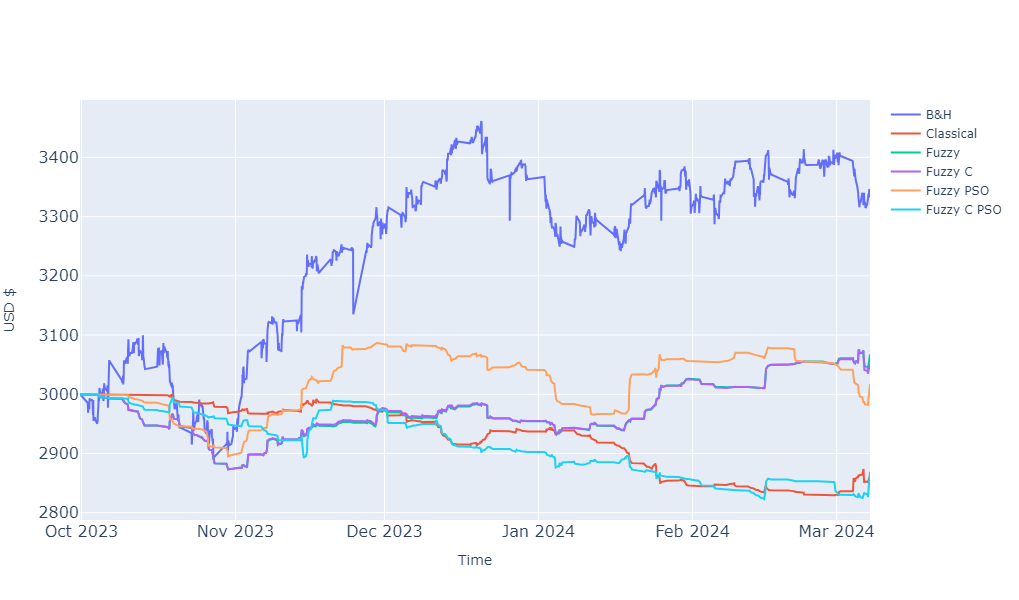
\includegraphics[width=\textwidth]{images/rsi-bb/stock-result.png}
    \caption{ความเปลี่ยนของเงินลงทุนของตัวชี้วัด RSI-BB ในตลาดหุ้น NASDAQ}
\end{figure}

\section{การทดลองกับตลาดที่มีทิศทางไม่แน่นอน และตลาดขาลง}

\section{การใช้กรอบของเวลาที่ต่างกัน (1h กับ 1d)}